\section{本文组织结构}
本文聚焦隐私保护机器学习中的效率和安全问题,其结构安排如下:
%
第1章介绍了隐私保护机器学习的背景知识,阐述了机器学习中隐私保护的重要性;
第2章介绍了隐私保护机器学习的研究现状,重点介绍了拆分学习、密码学方法,以及密码学和非密码学的混合方法三大研究方向;
第3章针对拆分学习的通信效率问题,提出了一种新的拆分学习通信压缩方法;
第4章针对拆分学习的隐私问题,提出了一种拆分学习隐私保护方法;
第5章针对密码学方法的效率问题以及其他方法的中间结果隐私暴露问题,提出了一种混合秘密分享和随机排列的安全神经网络框架;
第6章在第5章的基础上针对大语言模型进行优化,提出了一套高效的大语言模型隐私推断框架;
第7章对全文进行了总结,并提出了几个未来可能的研究方向。
%
\autoref{fig:overview}简明地呈现了本文的组织结构。

\begin{figure}[h!]
    \centering
    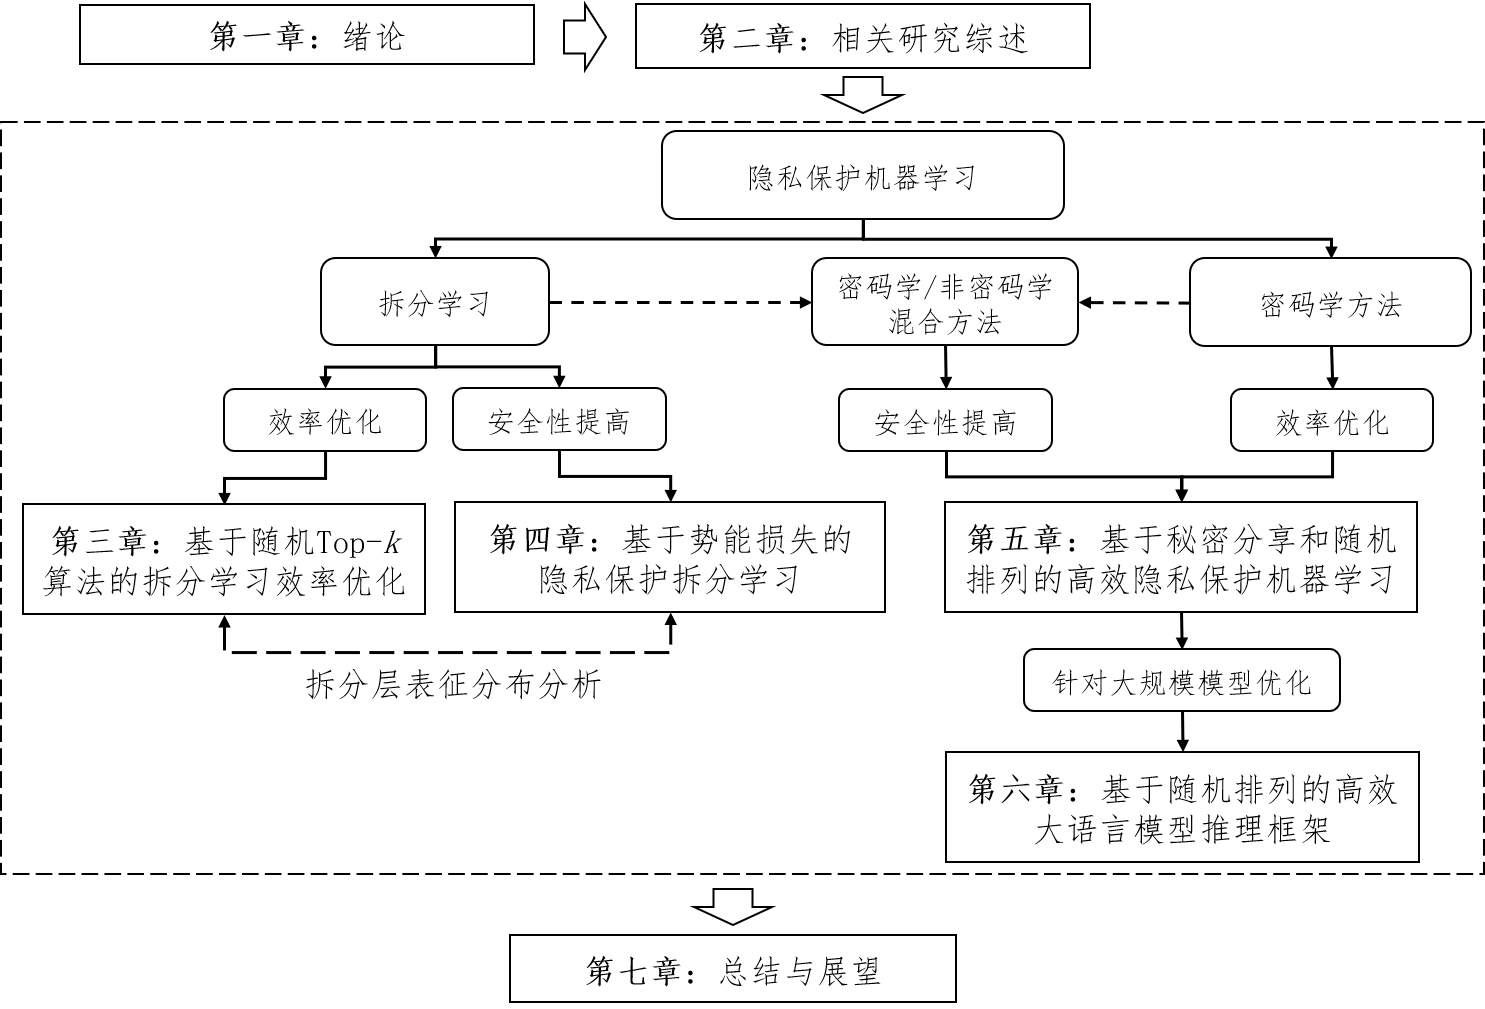
\includegraphics[width=\linewidth]{Z_Resources/article_overview.png}
    \caption{本文的组织结构示意图}
    \label{fig:overview}
\end{figure}